\section{Unified Action-Level Formulation and Scheduling}

We first formulate the entire workflow at the action level in \S\ref{sec:design_modeling}.
Our formulation unifies heterogeneous external resource types and diverse tool types.
Then we introduce our elastic resource scheduling algorithm in \S\ref{sec:design_scheduling}.
% Several primitives are defined to acquire and interpret these arguments.

\subsection{Action Formulation}
\label{sec:design_modeling}

\paraf{Vectorized Resource Cost Modeling.} 
At first, to enable unified action-level scheduling, we need a clear and unified representation of the resource cost.

Given an action, $a_i$, it may consume multiple types of resource simultaneously. For example, an action of the DeepSearch RL task may involve parallel or subsequent queries to multiple websites, where each website has a unique API quota and is considered as a different resource type.
An action of the AI coding task involves not only CPUs but also memory.
Thus, the cost of an action is represented as a multi-dimensional vector, denoted as $C_i = (c_{i,0}, c_{i,1},...,c_{i,k-1})$, where $k$ refers to the number of resource types managed by \sysname.
The vector enables joint consideration of multiple resource constraints during scheduling and allocation.
Each dimension of the vector corresponds to the consumption of one type of resource managed by \sysname (including CPU, GPU, memory, GPU memory, network bandwidth, and external API quotas).

Importantly, the cost for each resource type is not a static value.
For actions that are elastic to the resource quantity, the cost is specified as a range between the minimum and maximum feasible resource usage.
Even more sophisticated, for some specific tasks like reward services occupying multiple GPUs, the allowed unit of resource is discrete (e.g. 1, 2, 4, 8).
Therefore, the $c_{i,j}$ in $C_i$ has a specific constraint, representing its all possible resource quantity.
This formulation allows the scheduler to flexibly adjust resource allocation without violating feasibility constraints or introduce some priors to narrow the search space during scheduling.

\iffalse
Given an action, $a_i$, it may consume multiple types of resource simultaneously. For example, an action of the deep search RL task may involve parallel or subsequent queries to multiple websites; A CPU-intensive action may be constrained not only by the number of available CPU cores but also by the remaining system memory. 
Thus, the cost of an action is represented as a multi-dimensional vector, denoted as $C_i = (c_{i,0}, c_{i,1},...,c_{i,k-1})$, where $k$ refers to the number of resource types managed by the system, enabling joint consideration of heterogeneous resource constraints during scheduling and allocation. Each dimension of the vector corresponds to the consumption of one type of resource managed by the system (e.g., CPU cores, GPU memory, system memory, network bandwidth, external API quotas).

Importantly, the cost for each kind of resource is not just a static value. For actions that are scalable with respect to a given resource, the cost is specified as a range, denoted by a lower bound and an upper bound, representing the minimum and maximum feasible resource usage. Even more sophisticatedly, for some specific tasks like those occupying multiple GPUs, the allowed unit of resource is discrete (e.g. 1, 2, 4, 8). Therefore, each component $c_{i,j}$ in the vector $C_i$ is denoted as a data structure defined by the corresponding resource manager, which incorporates all possible consumption of resources. 
This formulation allows the scheduler to flexibly adjust resource allocation without violating feasibility constraints or introduce some priors to narrow the search space during scheduling.
\fi

\parabf{Elasticity Modeling.} For elastic actions, an additional argument is introduced to describe their elastic behavior.
In terms of a specific resource, its elasticity is described by a mapping from the $m$ units of the resources to a elastic ratio between 0 and 1. And the function satisfies the following:
\begin{equation}
\label{equ:scale}
\begin{aligned}
% a.\text{getDur}(m) = \frac{T_{ori} - T_{invar}}{S(m) * m} + T_{invar},
a.\text{getDur}(m) = \frac{T_{ori}}{E(m) * m}\quad (0<E(m)\le1),
\end{aligned}
\end{equation}
where $T_{ori}$ refers to the execution duration with a single unit.
%and $T_{invar}$ refers to the part of original duration that is invariant to the allocated units.

To simplify modeling and optimization, we assume that among all resource types consumed by an action, only one resource type is the key elasticity resource. 
This assumption is reasonable in many practical scenarios.
For instance, GPU-based actions require sufficient GPU memory for execution, but their execution latency is primarily determined by the degree of parallelism.
Under this assumption, the elasticity of an action is defined as a mapping from the usage of the key resource type, $S(m)~( m \in c_{i, key},~0\le key < k)$, which quantifies how the execution duration changes with the allocated amount of the key resource.

\parabf{Execution Duration Modeling.}
To prepare for the elastic scheduling algorithm, it is essential to incorporate execution durations into the action specification in addition to elasticity.
Therefore, we introduce the original execution duration and normalize it with a single unit, as aforementioned in Eq.\ref{equ:scale}, for actions whose execution duration is profileable. 
These profiles, along with the definition of elasticity, allow the system to estimate the time cost under different resource allocations, which is essential for optimizing scheduling decisions and balancing performance with resource efficiency. 


\subsection{Elastic Resource Scheduling}
\label{sec:design_scheduling}

An elastic resource scheduling algorithm for actions, motivated by the action-level resource allocation and scheduling, is required to guarantee the efficiency under finite resources. 

We first formulate the action completion time (ACT) as the optimization objective of the scheduling algorithm. 
Analogous to the job completion time (JCT), ACT is decomposed into: (1) the duration when the action queuing to be scheduled; (2) the execution duration of the action. The scheduling objective is therefore to find the resource allocation among several actions that minimizes the sum of ACTs:
\begin{equation}
\label{equ:obj}
\begin{aligned}
 \text{Objective:} \quad {\text{minimize}} ~ ACTs =\sum_{0\leq i < N} (T^q_{i} + T_i),
\end{aligned}
\end{equation}
where $N$ denotes the number of actions in the waiting queue at the scheduling time, $T_i$ denotes the actual execution duration of $ith$ action, and $T^q_{i}$ denotes its queuing duration.

Specific to the elastic scheduling algorithm, the problem consists of two coupled problems: (1) determining the execution order of actions in the waiting queue, and (2) determining how many units of resources to allocate for each action, both of which are non-trivial. 
To narrow the search space and align with the key observation of this paper, resource over-provisioning, we mainly focus on the second problem. %, while adopting a trivial algorithm for the first is enough. 
Since all actions lie on the critical path of their corresponding trajectories, agentic RL training is highly sensitive to the issue of starvation (a starved action may invalidate the entire trajectory). Therefore, we choose a First-Come First-Served (FCFS) policy to determine the scheduling order.
Our scheduling algorithm can work with other ordering algorithms.

The second problem is a classical problem: allocating finite units of resources among several elastic jobs and minimizing the total JCTs, which is NP-hard~\citep{bruno1974scheduling}. As discussed in \S~\ref{sec:background_op}, the quite short window of scheduling necessitates a heuristic solution, and the heterogeneity of both resource types and job patterns requires generalizability. Accordingly, we propose a unified heuristic scheduling algorithm, primarily based on a greedy eviction algorithm with approximated objective, as shown in Algorithm~\ref{alg:ersa}.

\iffalse
\begin{algorithm}[t!]
\caption{Elastic Resource Scheduling Algorithm.}\label{alg:ersa}
    \begin{footnotesize}
    \begin{algorithmic}[1]
        \Require Actions in the waiting queue $W$, resource status $R = \{R_0, ..., R_{k-1}\}$, historical information $\alpha = \{\alpha_0,...\alpha_{k-1}\}$
        \State $Selected \gets \varnothing$
        \State $C \gets W[:n],~n=\max\{i \mid R.\text{accommodate}(W[:i])\}$ \algcomment{Get candidates}
        \For{$j = 0 \rightarrow k-1 $} \algcomment{Process actions sharing key scalability resource $R_j$}
            \State $C_j \gets C.\text{split}(R_j)$
            \If{ $\forall a_{i} \in C_j$: ($S_{i}$ is None or $S_{i} \equiv 0$)}
            \State $Selected+= C_j$;~\textbf{continue} \algexit{Case\textcircled{1}: scalability unknown or zero}
            \EndIf
            
            \State $\alpha_j \gets \text{updateAlpha}(R_j, \alpha_j)$ \algcomment{Avoid overly aggressive allocation}
            \For{$\forall a_i \in C_j$} ~ $c_{i,j}^{max} \gets \alpha_j * c_{i,j}^{max} + (1-\alpha)* c_{i,j}^{min}$   
            \EndFor
            %\textcircled{2}:如果scalable action的execution duration未知
            \If{$\exists a_{i} \in C_j$: ($S_{i} > 0$ and $T_{i}$ is None)}
            % \State $Selected += C_j[:n],~n=\max\{: R_j >=(c_{i,j}^{max}\quad\forall a_i \in C_j[:k])\};$
            \State $Selected += C_j[:n],~n = \max \left\{ n \mid R_j \ge \sum_{i < n} c_{i,j}^{max} \right\}$;
            \State \textbf{continue} \algexit{Case\textcircled{2}: execution duration of scalable tasks unknown}
            \EndIf
            %\textcircled{3}:scalability和对应的execution duration均已知
            \State $obj \gets \text{getApproximatedObjective}(C_j, R_j)$ \algcomment{Initialize objectives}
            \For{$k = 1 \rightarrow |C_j|$} \algcomment{Greedily evict the last action and compare}
            \State $newObj \gets \text{getApproximatedObjective}(C_j[:-k], R_j)$
            \If{$newObj >= obj$} \textbf{break}
            \Else~~$obj \gets newObj$
            \EndIf
            \EndFor
            \State $Selected += C_j[:-k+1]$;~\textbf{continue}  \algexit{Case\textcircled{3}: Resource $R_j$ over}
        \EndFor
        \Return $Selected$
    \end{algorithmic}
    \end{footnotesize}
\end{algorithm}
\fi
% without scalability:
% without duration:


\begin{algorithm}[t!]
\captionof{algorithm}{Elastic Resource Scheduling Algorithm.}\label{alg:ersa}
    \begin{footnotesize}
    \begin{algorithmic}[1]
        \Require Actions in the waiting queue $W$, vectorized resource status $R = (R_0, ..., R_{k-1})$
        \State $Selected \gets \varnothing$
        \State $C \gets W[:n],~n=\max\{i \mid R.\text{accommodate}(W[:i])\}$ \algcomment{Get candidates}
        \For{$j = 0 \rightarrow k-1 $} \algcomment{Process actions sharing key elasticity resource $R_j$}
            \State $C_j \gets C.\text{split}(R_j)$
            \If{ $\forall a_{i} \in C_j$: ($E_{i}$ is None or $S_{i} \equiv 0$)} \algcomment{if elasticity unknown}
            \State $Selected+= C_j$;~\textbf{continue} \algcomment{or zero, directly continue}
            \EndIf
            %\textcircled{3}:scalability和对应的execution duration均已知
            \State $obj \gets \text{getApproximatedObjective}(C_j, R_j)$ \algcomment{Initialize objectives}
            \For{$t = 1 \rightarrow |C_j|$} \algcomment{Greedily evict the last action and compare}
            \State $newObj \gets \text{getApproximatedObjective}(C_j[:-t], R_j)$
            \If{$newObj >= obj$} \textbf{break}
            \Else~~$obj \gets newObj$
            \EndIf
            \EndFor
            \State $Selected += C_j[:-t+1]$;~\textbf{continue} 
        \EndFor
        \Return $Selected$
    \end{algorithmic}
    \end{footnotesize}
\end{algorithm}


Each time the scheduling algorithm is invoked, we first select the first $n$ actions from the waiting queue as candidates $C$ (due to FCFS), ensuring that vectorized resource constraints $R = (R_0, ..., R_{k-1})$ are satisfied with each action allocated with least-required resource units, i.e.,
$$
R_j \ge \{c_{0,j}^{min}, ...,c_{n-1,j}^{min}\},
$$
where $\ge$ indicates that not only the remaining units of $j$th resource type is no smaller than the sum of the minimum requirements $c_{i,j}^{min}$, but also the current status in terms of its actual topology can accommodate all these candidates (Line 1-2).
We then split the candidates into several groups according to the key elasticity resource (\S~\ref{sec:design_modeling}), and respectively apply the elastic allocation algorithm on each resource type. Granted by the assumption that an action’s elasticity is dominated by a single resource type, scaling an action along this resource does not affect the allocation of other resources (Line 3-4).
For each resource type, the algorithm selects a subset of candidates and determines their allocated units.


\iffalse
\textit{Case\textcircled{1}}~(Line 5-6): The scalability of these actions is zero or difficult to model. We believe no effective optimization is possible in this case, and each action is allocated only its minimum required resource units.  

\textit{Case\textcircled{2}}~(Line 7-11): Although the scalability of scalable tasks can be modeled with some priors, the execution durations of these actions are still unavailable. We introduce a historical indicator $alpha$ to characterize the scarcity of this resource type in recent periods. Specifically, scarcity is defined as the ratio between: 1) the maximum number of actions that can be accommodated under the current system state (remaining units plus currently executing actions), and 2) the maximum number under the system-wide capacity. 
Furthermore, we recap the maximum allocatable units for each action by interpolating between its minimum and maximum resource requirements using $alpha$, in order to avoid overly aggressive resource allocation, leading to prolonged queuing time under bursty workloads.
\fi

% \begin{algorithm}[t!]
% \caption{ACTs Approximation.}
%     \begin{footnotesize}
%     \begin{algorithmic}[1]
%     \Require The waiting queue of actions $W$, the executing queue $E$, the $depth$ of performing approximation of objective
%         \Function{getApproximatedObjective}{$C_j, R_j$}
%             \State $AC_j \gets W.\text{split}(R_j) - C_j$ \algcomment{Actions to be scheduled the next step}
%             \State $exactObj,~newHeap \gets \text{DPArrange}(R_j, C_j)$
%             \State $approxObj \gets newHeap.\text{estimate}(AC_j)$
%             \State \Return $exactObj + approxObj$
%         \EndFunction

%         \Statex
        
%         \Function{estimate}{$heap, C$}
%         \State $obj \gets \inf, ~heap \gets \text{copy}(heap)$
%         \For{$d=1 \rightarrow depth$}
%         \State $T_0 \gets C[0].\text{getDur}(d),~ts \gets heap.\text{pop}()$
%         \State $tmpObj \gets 0,~tmpHeap \gets \text{copy}(heap)$
%         \State $tmpObj+=ts+T_0,~tmpHeap.\text{push}(ts+T_0)$
%         \For{$i=1 \rightarrow |C|$}
%         \State $T_i \gets C[i].\text{getDur}(),~ts \gets heap.\text{pop}()$
%         \State $tmpObj+=ts+T_i,~tmpHeap.\text{push}(ts+T_i)$
%         \EndFor
%         \If{$tmpObj < obj$}~$obj \gets tmpObj$
%         \EndIf
%         \EndFor
%         \State \Return $obj$
%         \EndFunction
%     \end{algorithmic}
%     \end{footnotesize}

% \end{algorithm}

For scalable actions that both elasticity and execution durations are known, we propose a greedy algorithm by approximating the objectives, ACTs, during the decision process. First, we schedule all candidates $C_j$ using their minimum resource requirements and compute the initial objective.
Second, we iteratively evict the last action from candidates $C_j$ and reassign its resources to the remaining actions. For each reduced candidate set $C_j[:t]$, we compute the optimal resource allocation and the corresponding objective. Once further eviction fails to reduce the objective, which means that evicting this action and scaling the left candidates fails to optimize the ACTs, the greedy algorithm terminates. 

As for objective approximation (the pseudo code is shown in Appendix), we decompose it into two parts, i.e., the ACTs of the candidates and the ACTs of the remaining actions in the waiting queue. Because the candidates are to be scheduled at once, their ACTs are computed exactly using their determined allocations. We employ a topology-agnostic dynamic programming (DP) algorithm that is applicable to heterogeneous resource topologies, termed as DPArrange in the pseudo code. This algorithm, provided in Appendix~\ref{app:udp}, resolves the optimal discrete allocation among these scalable candidates and generates the updated completion heap according to the allocation.
% , while the topology-aware variant is introduced in following \S~\ref{}.
However, ACTs of the remaining actions are influenced by the allocation strategy ahead of them. It is intractable to recursively compute the best allocation and attain the optimal objective for these actions. Instead, we simplify the process and estimate their ACTs by assigning minimum resources and sequentially inserting them into the completion heap.

Notably, to approximate the objective more precisely, we introduce a parameter $depth$, which expands the search space by allowing the first remaining action to explore multiple allocation choices. In practice, setting $depth=2$ or $3$ is sufficient. Moreover, the conditions require known execution durations only for scalable actions, rather than all actions. This is because, during greedy eviction of candidates, the durations of non-scalable actions remain constant, and do not affect the relative comparison of objectives.
Although their exact execution durations affect the completion heap, it is acceptable to be approximated by historical averages, due to the fact that scalable actions typically last for much longer duration than non-scalable ones and dominate the evolution of the completion heap. The computational complexity of this algorithm is dominated by the implementation of the DP algorithm. Using the classical implementation for common topologies, the overall complexity is $O(kn^2m^2)$, where $n$ refers to the number of candidates and $m$ refers to the remaining units of a resource type.

As for the non-scalable resource or the actions whose elasticity are unknown, the algorithm directly select these candidates and allocate them with least-required units, while guaranteeing the vectorized resource constraints satisfied.




\section{Heterogeneous Resource Managers}
\label{sec:design_resource_managing}

While providing a unified abstraction and scheduling algorithm, achieving \textbf{Breakdown} \& \textbf{Pool} (\S\ref{sec:background_opp}) additionally requires resource-specific management policies. 
In particular, \textbf{Breakdown} focuses on releasing resources while preserving execution states or enabling fast restoration, i.e., efficient context switching, as well as supporting elastic degrees of parallelism for each action.
\textbf{Pool} emphasizes the design of resource allocation that mitigate fragmentation and improve parallel efficiency, thereby backing up the unified elastic scheduling framework.
As discussed in Section~\ref{sec:background_opp}, heterogeneous resources differ significantly in both characteristics and topologies.
We therefore design specialized resource managers for different resource types, including CPUs, GPUs, and other basic resources.
%, and present their design principles.


\subsection{Basic Resource Manager}
For external resources that cannot be scaled up, such as website quotas and request QPS limits, we introduce a \emph{Basic Resource Manager} to prevent contention and violations of resource constraints.
This manager supports two consumption patterns: concurrency-based (limiting the maximum concurrent usage) and quota-based (limiting the total usage in a period).
It also defines a set of basic interfaces that can be inherited and selectively overridden to support action-level scheduling and unified resource management.

\subsection{CPU Manager via AOE}


In current cloud CPU clusters, the combination of Kubernetes (k8s) and Docker is the de facto standard, where Docker provides environment isolation and k8s performs cluster-level resource management. However, designed for long-running cloud services, k8s incurs substantial scheduling overhead 
and only manages resources at the granularity of pods. Resource quotas are fixed at pod creation time\footnote{In-place resizing is not yet available in stable releases and introduces unacceptable latency even in nightly versions.}, which leads to over-provisioning within trajectories in agentic RL workloads.
To address this limitation, we introduce a CPU management mechanism termed \emph{allocate-on-execution (AOE)}, which directly interacts with containers and prepares for fine-grained CPU allocation.

\parabf{Breakdown in CPU Manager.} 
AOE leverages Docker’s \texttt{update} interface to modify a container’s cgroup configuration on demand, including parameters like \texttt{cpulimit} and \texttt{cpuset}. Before each invocation of \texttt{docker.exec()}, CPU Manager updates the container’s cgroup according to the resource units assigned by the scheduling algorithm. Docker then forks a process under the updated cgroup to execute the action. After execution, the process terminates and the allocated CPU resources are reclaimed.
Notably, to preserve the long-lived state of each environment, the memory allocated to each container is preserved, which is acceptable in modern clusters with abundant memory capacity.

Adjusting cgroup configuration alone is insufficient to achieve elastic DoP, since not all elastic actions innately are allowed for parallel in actual. Therefore, we should ensure the elasticity of certain actions when constructing RL datasets or submitting actions. 
% \zhl{is elasticity suitable for ``Breakdown''? maybe better in ``Pool'', or a new primitive? }
For example, in code generation tasks, test cases can be efficiently executed in parallel, yet the testing commands provided in existing datasets typically support only single-process execution. As most test commands rely on the library \texttt{pytest}, we replace \texttt{pytest} with \texttt{pytest -n \$\{parallel\_num\}} and dynamically set \texttt{parallel\_num} at runtime to enable parallel execution.


\parabf{Pool in CPU Manager.}
The design of resource allocation in CPU clusters is relatively straightforward. Since CPU cores and CPU memory are tightly coupled, CPU Manager jointly manages these two resource types. For CPU allocation, the manager not only determines the number of cores assigned to each action but also explicitly specifies the set of cores used for parallel execution. Each core is exclusively occupied by a single action at any time, preventing interference across actions.
In addition, parallel efficiency is affected by inter-core communication overhead, which depends on the physical distances between cores on the chip. Therefore, when allocating CPU cores for elastic actions, CPU Manager prioritizes selecting cores within the same Non-Uniform Memory Access (NUMA) node.


When the first action of a trajectory is invoked, CPU Manager filters nodes that have sufficient resources—namely, enough CPU cores for the action and sufficient memory for the entire trajectory—and selects one node according to a CPU memory load-balancing policy. All subsequent actions within the same trajectory are then constrained to execute on the selected node.
Although CPUs across different nodes cannot cooperate for parallel execution, modern cloud CPU nodes typically provide 128 cores or more. This capacity is large relative to the number of CPU cores allocated per action, and as a result, fragmentation of CPU cores is generally not severe in practice. Therefore, CPU Manager independently performs the scheduling algorithms for each node.

\begin{figure}[t]
    \centerline{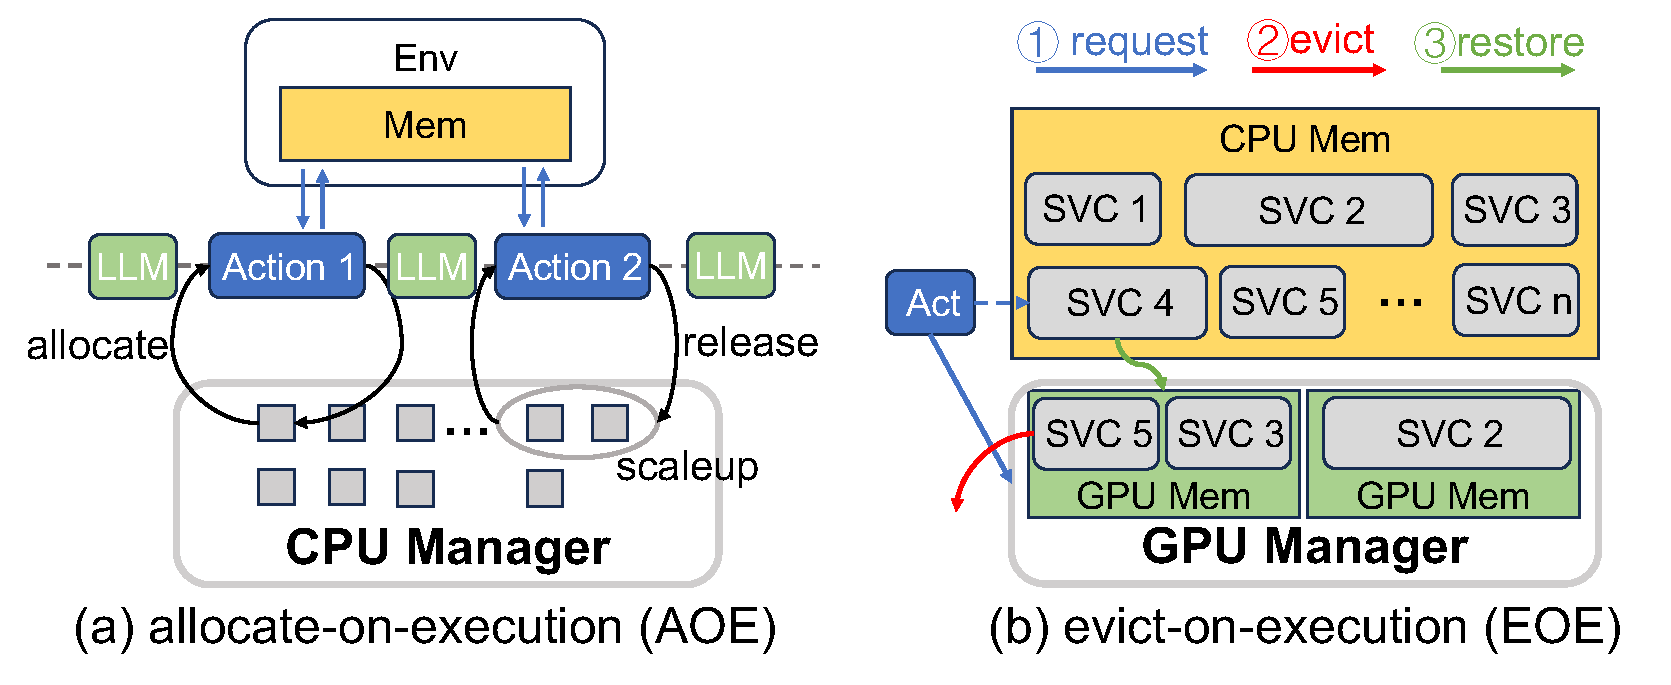
\includegraphics[width=0.8\linewidth]{figures/manager.pdf}}
    \vspace{-0.1in}
    \caption{Heterogeneous resource management.}
    \label{fig:design_manager}
    \vspace{-0.15in}
    \end{figure}

\subsection{GPU Manager via EOE}
Compared with Docker-based CPU environments, long-lived services on GPU clusters incur significantly higher setup overhead. For example, a reward model service must compile kernels, establish communication groups, and, most critically, load model parameters into GPU memory~\citep{zhang2025blitzscale,lou2025hydraserveminimizingcoldstart}.
Moreover, GPU memory is both scarce and heavily contended, preventing all services from being persistently cached. Relying solely on CPU-memory caching would introduce prohibitive restoration overhead. We adopt an \emph{evict-on-execution (EOE)} mechanism to reduce context-switch overhead, and design corresponding resource allocation strategies to mitigate resource fragmentation and service dithering.


\parabf{Breakdown in GPU Manager.} 
Upon initialization, GPU Manager iteratively prepares all required services by deploying them on each feasible group of GPUs and backing up their states in CPU memory. When an action requests a service, GPU Manager allocates a set of GPUs with required units and checks whether the requested service is already resident in GPU memory. If so, the action is executed immediately.
Otherwise, the GPU Manager restores the service from CPU memory, evicting cached services from GPU memory as necessary until sufficient memory is available for exclusive execution. After the action completes, the restored service remains cached in GPU memory until it is evicted at a later time. 
Although eviction and restoration inevitably introduce additional latency, we observe that GPU memory states of many services remain unchanged across invocations. As a result, eviction does not require writing service states back to CPU memory; it is sufficient to release the occupied GPU memory while keeping an invariant copy in CPU memory.
Regarding the overhead of restoring services from CPU memory, prior work~\citep{zhang2025blitzscale,xiang2025aegaeon} has shown that this cost can be effectively reduced, making the overhead acceptable in practice.

Elastic DoP is naturally supported under EOE by treating different DoP configurations of a service as distinct services. An action requesting a service can be routed to any instance of arbitrary DoP, and relies on the scheduling algorithm to make decision.
Notably, EOE guarantees that all cached services have sufficient GPU memory to serve actions, while GPU allocation enforces that at most one action executes on each GPU at any time. This design enables a GPU cluster to host multiple services efficiently for agentic RL training.


\parabf{Pool in GPU Manager.}
The specialized topology of GPU clusters—characterized by fewer devices per node and strong demands for parallel execution—necessitates careful mitigation of GPU fragmentation.
We adopt a multi-level cell structure~\citep{zhao2020hived} to organize and manage GPU resources.
Targeting common DoPs, a legal allocation set, termed \emph{chunk}, is defined as a contiguous GPU interval $(start, end)$ satisfying:
$$
end - start = 2^a~~ \text{and}~~ start | 2^a\quad (a \in \{0,1,2,3\}),
$$
where $a$ refers to the level of this chunk.
Initially, each GPU node is represented as a single available chunk $(0, 8)$ with level 3. When allocating $m$ GPUs, where $2^{a-1} < m \le 2^a$, GPU Manager traverses available chunks in the order of levels and selects the smallest chunk with level $b~(b\ge a)$. If $b > a$, GPU Manager splits the chunk into several legal chunks accordingly, and the resulting chunk is returned.
In addition, GPU Manager applies a least-recently-used (LRU) eviction policy, to reduce dithering of service cache. When multiple chunks of the same level are available, preference is given to the chunk that already caches the requested service.

All interfaces required by the unified scheduling algorithm and related to the topology of external resources are overloaded in GPU Manager, particularly the topology-agnostic DP algorithm, which is detailed in Appendix~\ref{app:udp}.